\documentclass[11pt]{article}

\usepackage[letterpaper,margin=0.75in]{geometry}
\usepackage[T1]{fontenc}
\usepackage{lmodern}
\usepackage{microtype}
\usepackage{amsmath,amssymb}
\usepackage{booktabs}
\usepackage{tabularx}
\usepackage{array}
\usepackage{enumitem}
\usepackage{graphicx}
\usepackage{xcolor}
\usepackage{tikz}
\usetikzlibrary{arrows.meta,positioning,calc}
\usepackage{fancyhdr}
\usepackage{titlesec}
\usepackage{hyperref}
\usepackage{listings}
\usepackage{caption}

% ---------------- Typography and colors ----------------
\definecolor{accent}{HTML}{461D7C}
\definecolor{rulegray}{HTML}{666666}
\definecolor{lightgray}{HTML}{F4F4F4}
\definecolor{linkblue}{HTML}{1F4E79}

\hypersetup{
    colorlinks=true,
    linkcolor=linkblue,
    urlcolor=linkblue
}

\setlength{\parindent}{0pt}
\setlength{\parskip}{5pt}
\setlist[itemize]{leftmargin=1.45em,itemsep=2pt,topsep=2pt}
\setlist[enumerate]{leftmargin=1.6em,itemsep=2pt,topsep=2pt}

\titleformat{\section}
  {\large\bfseries\color{accent}}
  {\thesection.}{0.55em}{}
\titleformat{\subsection}
  {\normalsize\bfseries}
  {\thesubsection}{0.5em}{}
\titlespacing*{\section}{0pt}{12pt}{5pt}
\titlespacing*{\subsection}{0pt}{8pt}{3pt}

\pagestyle{fancy}
\fancyhf{}
\lhead{CSC 4501: Computer Networks}
\rhead{QuantumNet Course Project}
\cfoot{\thepage}
\renewcommand{\headrulewidth}{0.4pt}

\captionsetup{font=small,labelfont=bf}

\lstset{
  basicstyle=\ttfamily\small,
  backgroundcolor=\color{lightgray},
  frame=single,
  rulecolor=\color{black!20},
  breaklines=true,
  columns=fullflexible,
  showstringspaces=false,
  xleftmargin=4pt,
  xrightmargin=4pt,
  aboveskip=5pt,
  belowskip=5pt
}

\newcommand{\points}[1]{\hfill\textbf{[#1 points]}}

\begin{document}

% ---------------- Header ----------------
\begin{center}
    {\Large\bfseries QuantumNet: Routing and Congestion in a Distributed Quantum Network}\\[4pt]
    {\normalsize Course Project -- CSC 4501: Computer Networks}\\[6pt]
    \rule{\textwidth}{0.6pt}
\end{center}

\begin{center}
\small
\begin{tabularx}{0.90\textwidth}{@{}>{\bfseries}p{0.25\textwidth} X@{}}
Course & CSC 4501: Computer Networks \\
Project weight & 10\% of the course grade \\
Implementation & Python \\
Network model & 6 QPUs connected by 9 bidirectional links \\
Prerequisite & Basic Python programming and graph/routing concepts \\
Prior quantum knowledge & None required \\
\end{tabularx}
\normalsize
\end{center}

\vspace{4pt}
\textbf{Project objective.}
This project studies routing and congestion in a simplified distributed quantum network. The quantum setting provides the application context; the technical work remains centered on computer-networking concepts: weighted graphs, shortest paths, reliability, finite link capacity, queueing, congestion, throughput, and controlled experimental comparison.

\textbf{Important.}
You are not expected to simulate quantum gates, qubits, quantum states, or quantum circuits. Treat an \emph{entanglement request} as an end-to-end connection request between two network nodes.

\section{System Model and Minimal Background}

A distributed quantum system can be viewed as several quantum processing units (QPUs) connected through communication links. For this project, each QPU is a graph node and each physical link is a graph edge. A request must be routed from a source QPU to a destination QPU through one or more links.

Each link has three properties:
\begin{itemize}
    \item \textbf{Delay} $d_e$: service time required to use link $e$.
    \item \textbf{Success probability} $p_e$: probability that the link-level connection attempt succeeds.
    \item \textbf{Capacity} $c_e$: maximum number of requests that can simultaneously use the link.
\end{itemize}

\begin{figure}[ht]
\centering
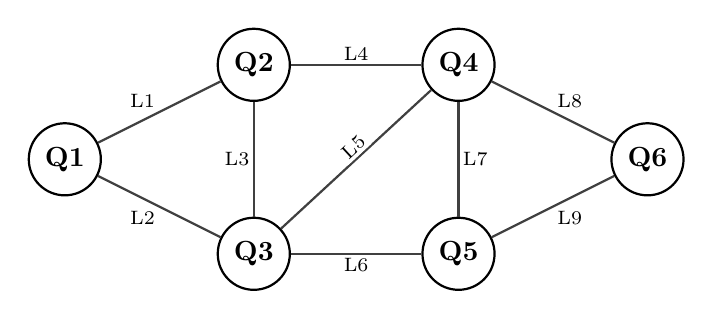
\begin{tikzpicture}[
    qpu/.style={circle,draw=black,thick,minimum size=9mm,font=\bfseries},
    edge/.style={draw=black!75,thick},
    eid/.style={fill=white,inner sep=1.2pt,font=\scriptsize}
]
\node[qpu] (q1) at (0,1.8) {Q1};
\node[qpu] (q2) at (2.4,3.0) {Q2};
\node[qpu] (q3) at (2.4,0.6) {Q3};
\node[qpu] (q4) at (5.0,3.0) {Q4};
\node[qpu] (q5) at (5.0,0.6) {Q5};
\node[qpu] (q6) at (7.4,1.8) {Q6};

\draw[edge] (q1)--node[eid,above left] {L1} (q2);
\draw[edge] (q1)--node[eid,below left] {L2} (q3);
\draw[edge] (q2)--node[eid,left] {L3} (q3);
\draw[edge] (q2)--node[eid,above] {L4} (q4);
\draw[edge] (q3)--node[eid,pos=.53,above,sloped] {L5} (q4);
\draw[edge] (q3)--node[eid,below] {L6} (q5);
\draw[edge] (q4)--node[eid,right] {L7} (q5);
\draw[edge] (q4)--node[eid,above right] {L8} (q6);
\draw[edge] (q5)--node[eid,below right] {L9} (q6);
\end{tikzpicture}

\vspace{4pt}
\footnotesize
\begin{tabular}{cccc@{\hspace{12mm}}cccc}
\toprule
Link & Endpoints & $d_e$ (ms) & $p_e$ & Link & Endpoints & $d_e$ (ms) & $p_e$ \\
\midrule
L1 & Q1--Q2 & 8 & 0.96 & L6 & Q3--Q5 & 9 & 0.91 \\
L2 & Q1--Q3 & 5 & 0.82 & L7 & Q4--Q5 & 4 & 0.95 \\
L3 & Q2--Q3 & 4 & 0.88 & L8 & Q4--Q6 & 8 & 0.90 \\
L4 & Q2--Q4 & 7 & 0.93 & L9 & Q5--Q6 & 6 & 0.94 \\
L5 & Q3--Q4 & 5 & 0.86 & & & & \\
\bottomrule
\end{tabular}
\normalsize
\caption{Project topology. Edge identifiers in the graph correspond to the link parameters shown below. Capacities are $c_e=2$ for all links except L2, for which $c_{\mathrm{L2}}=3$. The complete topology is provided in \texttt{data/topology.json}.}
\label{fig:topology}
\end{figure}

The network contains six QPUs and nine bidirectional links. Multiple source--destination pairs therefore have several feasible routes. For example, a Q1-to-Q6 request can be routed through different intermediate nodes, and the path with the fewest hops need not have the lowest delay or the highest end-to-end success probability.

\section{Provided Repository Structure}

Students receive the following files:
\begin{lstlisting}
QuantumNet/
|-- data/
|   `-- topology.json
|-- student/
|   `-- starter.py
|-- requirements.txt
`-- PROJECT_SPEC.pdf
\end{lstlisting}

Complete only the numbered \texttt{TODO} sections in \texttt{starter.py}. Do not rename required functions. The topology file should not be modified for the required experiments.

\section{Project Tasks}

\subsection{Task 1: Network Topology Construction \points{10}}
Complete \texttt{load\_topology(...)}. Your implementation must read the provided JSON file, construct an undirected graph, preserve all edge attributes, verify $0<p_e\leq1$, verify $c_e\geq1$, and verify that the topology is connected.

\textbf{Required output:} a labeled topology figure comparable to Fig.~\ref{fig:topology}.

\subsection{Task 2: Traffic Generation \points{10}}
Complete \texttt{generate\_requests(...)}. Requests must arrive according to exponentially distributed inter-arrival times. Each request must contain a request ID, arrival time, source QPU, and destination QPU, with source and destination always different.

You will later vary the arrival rate to represent different levels of offered load.

\subsection{Task 3: Routing Policies \points{30}}
Implement the following four routing strategies.

\textbf{(a) Minimum-hop routing.} Select the path containing the fewest links.

\textbf{(b) Minimum-latency routing.} For path $P$,
\[
C_{\mathrm{latency}}(P)=\sum_{e\in P} d_e.
\]
Select the path with minimum total link delay.

\textbf{(c) Maximum-reliability routing.} Assuming independent link outcomes, the end-to-end success probability of path $P$ is
\[
P_{\mathrm{success}}(P)=\prod_{e\in P}p_e.
\]
Dijkstra's algorithm requires an additive path cost. Derive an additive link weight that produces the same ordering as maximizing the product above, and implement it in \texttt{edge\_weight(...)}. Your report must briefly justify the transformation.

\textbf{(d) Student-designed routing policy.} Design one additional metric that uses at least two link properties. You may combine delay, success probability, and/or capacity. State the formula, explain any parameters, and describe the behavior you expect from the metric before discussing the measured results.

\subsection{Task 4: Link Capacity and Queueing \points{15}}
Implement finite-capacity link service. Each link has $c_e$ simultaneous service slots. If all slots are occupied when a request reaches a link, the request must wait until the earliest slot becomes free.

Use the provided \texttt{LinkState} class. A min-heap of slot-availability times is recommended. For each request, track queue waiting time and end-to-end completion time. For each link, track the number of jobs served and utilization.

\begin{figure}[ht]
\centering
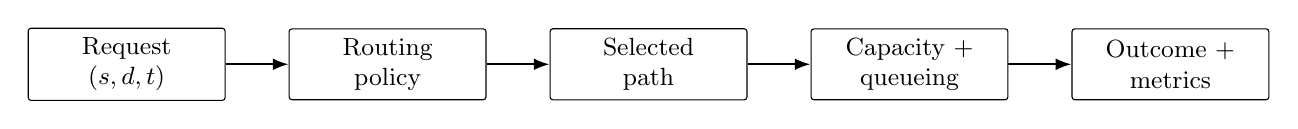
\begin{tikzpicture}[
    box/.style={draw=black,rounded corners=1pt,minimum height=9mm,minimum width=25mm,align=center,font=\small},
    arr/.style={-{Latex[length=2mm]},thick}
]
\node[box] (r) {Request\\$(s,d,t)$};
\node[box,right=8mm of r] (route) {Routing\\policy};
\node[box,right=8mm of route] (path) {Selected\\path};
\node[box,right=8mm of path] (queue) {Capacity +\\queueing};
\node[box,right=8mm of queue] (out) {Outcome +\\metrics};
\draw[arr] (r)--(route);
\draw[arr] (route)--(path);
\draw[arr] (path)--(queue);
\draw[arr] (queue)--(out);
\end{tikzpicture}
\caption{Simulation flow for each generated request. Routing selects a path; finite link capacity may introduce queueing; the simulator then records success/failure and performance metrics.}
\label{fig:flow}
\end{figure}

\subsection{Task 5: End-to-End Simulation and Metrics \points{20}}
Complete the main simulation loop. For every request:
\begin{enumerate}
    \item select a route using the chosen policy;
    \item process the links along that route in order;
    \item reserve link capacity and accumulate any waiting time;
    \item sample link success/failure using the provided success probability; and
    \item stop after the first failed link or record successful completion.
\end{enumerate}

The simulator must report, at minimum, request success rate, average end-to-end latency, average waiting time, average hop count, throughput, and per-link utilization.

Use the following definitions:
\[
\text{Success Rate}=\frac{N_{\mathrm{success}}}{N_{\mathrm{total}}},
\qquad
\text{Throughput}=\frac{N_{\mathrm{success}}}{T_{\mathrm{sim}}}.
\]

\subsection{Task 6: Experimental Evaluation and Technical Report \points{15}}
Evaluate all four routing policies under the following offered loads:
\[
0.02,\quad 0.05,\quad 0.10,\quad 0.15 \qquad \text{requests/ms}.
\]

For a given load, every routing policy must receive the \textbf{same request trace}. This controls the workload and makes the comparison fair.

Generate the following four plots:
\begin{enumerate}
    \item request success rate vs. offered load;
    \item average end-to-end latency vs. offered load;
    \item throughput vs. offered load; and
    \item average queue waiting time vs. offered load.
\end{enumerate}

Your analysis should explain the networking mechanisms behind the results. At minimum, discuss why the three baseline policies can select different paths, how congestion changes their relative behavior, which links become bottlenecks, and when your proposed policy performs well or poorly.

\section{Experimental and Reporting Requirements}

Use a fixed random seed in the final experiments. A typical run is:
\begin{lstlisting}
python starter.py --topology ../data/topology.json \
                  --output ../outputs/student_run \
                  --requests 500 --seed 42
\end{lstlisting}

The report should be approximately four pages, excluding references. Organize it as a short technical report rather than a question-by-question worksheet. A recommended structure is:
\begin{enumerate}
    \item \textbf{Introduction and System Model}: problem statement, topology, and link attributes;
    \item \textbf{Routing Methods}: three baselines and the student-designed policy;
    \item \textbf{Experimental Setup}: traffic generation, offered loads, metrics, and random seed;
    \item \textbf{Results and Discussion}: plots, bottlenecks, tradeoffs, and explanation of observed behavior;
    \item \textbf{Conclusion}: concise summary of the main findings.
\end{enumerate}

\section{Submission Checklist}

Submit one folder containing:
\begin{lstlisting}
submission/
|-- quantumnet.py
|-- summary.csv
|-- topology.png
|-- success_rate_vs_load.png
|-- latency_vs_load.png
|-- throughput_vs_load.png
|-- waiting_vs_load.png
`-- report.pdf
\end{lstlisting}

Your code must execute without manual changes after submission. Figures in the report must have axis labels, legends, and captions. Numerical results should be reproducible from the submitted code and fixed seed.

\section{Scope and Modeling Assumptions}

This project intentionally uses a simplified network model. The topology is static during each experiment, link success events are treated as independent, and no quantum-state simulation is performed. These assumptions keep the project focused on the computer-networking questions of route selection, reliability, capacity, queueing, congestion, and throughput.

\vfill
\begin{center}
\rule{0.78\textwidth}{0.4pt}\\[-1pt]
\textbf{Central question:} Is the shortest route still the best route when latency, reliability, and congestion must be considered together?
\end{center}

\end{document}
